
\documentclass[12pt,a4paper]{ctexart}
\usepackage[top=25mm,bottom=25mm,left=22mm,right=22mm]{geometry}
\usepackage{graphicx}
\usepackage{booktabs}
\usepackage{longtable}
\usepackage{hyperref}
\usepackage{xcolor}
\usepackage{amsmath}
\usepackage{amsfonts}
\usepackage{natbib}

\title{\textbf{因果推断框架下的多因子选股研究}\\\large 基于沪深300成分股的因果因子发现与样本外验证}
\author{ZCode 自动化研究}
\date{\today}

\begin{document}
\maketitle

\begin{abstract}
\noindent 本研究使用因果推断框架重新检验 A 股沪深300成分股中多因子选股的因子有效性。研究区分"因果因子"与"相关因子"，通过 PC 与 FCI 算法进行因果发现，采用 Double Machine Learning、工具变量法、前门调整与 Causal Forest 四种方法估计因果效应，并在 2018--2022 年训练集与 2023--2024 年测试集上验证因子衰减与组合表现。\\[6pt]
\textbf{核心发现}：部分传统 IC 显著因子（如 ROE）在因果推断中并不显著，存在伪因子风险。 因果显著因子包括：MOM20, MOM60, TURN20。 因果显著因子组合样本外夏普（0.2777）高于 IC 显著因子组合（-0.9302），支持因果因子更稳健的判断。\\[6pt]
\noindent\textbf{关键词：}因果推断；因子发现；Double Machine Learning；工具变量；前门调整；Causal Forest；样本外验证
\end{abstract}

\tableofcontents
\newpage

\section{引言}
传统多因子研究依赖横截面相关性（IC）筛选因子，但高 IC 未必意味着因果效应。若因子与收益由共同的市场情绪或宏观冲击驱动，则基于相关性的因子组合可能因套利而快速衰减。因果推断的目标是从观测数据中估计干预后的分布 $P(Y\mid do(D=d))$，而非 merely 条件期望 $P(Y\mid D=d)$。本研究将因果推断框架系统引入 A 股多因子选股，区分因果显著因子与相关因子，并验证其样本外稳健性。

\section{相关工作}
因果推断在金融学中的应用日益受到关注。\cite{pearl2009causality} 提出的因果图与 do-演算奠定了识别因果效应的形式化基础；\cite{chernozhukov2018double} 提出的 Double Machine Learning（DML）利用机器学习估计干扰函数并通过交叉拟合消除偏差；\cite{wager2018estimation} 的 Causal Forest 则进一步估计异质性处理效应（ITE）。\cite{lopezdeprado2018advances} 强调了金融机器学习中因果推断与样本外验证的重要性。\cite{harvey2016and} 指出因子挖掘中的多重检验问题，提示研究者需区分真实预测能力与伪相关。

\section{数据与因子定义}
本研究使用 2018-01-02 至 2024-12-31 的沪深300成分股日行情数据。共构建 11 个横截面选股因子，所有因子经行业/板块中性化、MAD 去极值与截面标准化处理。预测标签为 20 日持有期收益。

\begin{tabular}{cc}
\toprule
因子 & 含义 \\ 
\midrule
EP & 盈利收益率 Earnings Yield = 1/PE \\ 
BP & 账面市值比 Book-to-Price = 1/PB \\ 
MOM20 & 20日动量 (剔除最近1日) \\ 
MOM60 & 60日动量 (剔除最近1日) \\ 
ROE & 净资产收益率 \\ 
ROA & 总资产收益率 \\ 
VOL20 & 20日收益波动率 (年化) \\ 
TURN20 & 20日平均换手率 \\ 
LIQ20 & 20日平均成交量 (对数) \\ 
GROWTH & 净利润同比增长率 \\ 
REV5 & 5日短期反转 \\ 
\bottomrule
\end{tabular}

控制变量包括市值对数、20 日市场收益、市场波动率、市场趋势以及板块哑变量。

\section{因果发现}
\subsection{PC算法与FCI算法}
PC 算法假设无潜在混杂，使用 Fisher-Z 条件独立性检验（$\alpha=0.05$）学习 CPDAG。FCI 算法允许存在未观测混杂因子，输出 PAG（Partial Ancestral Graph）。由于金融数据中市场情绪、宏观冲击等未观测变量几乎必然存在，FCI 的结果比 PC 更保守、更诚实。

\begin{figure}[htbp]
\centering
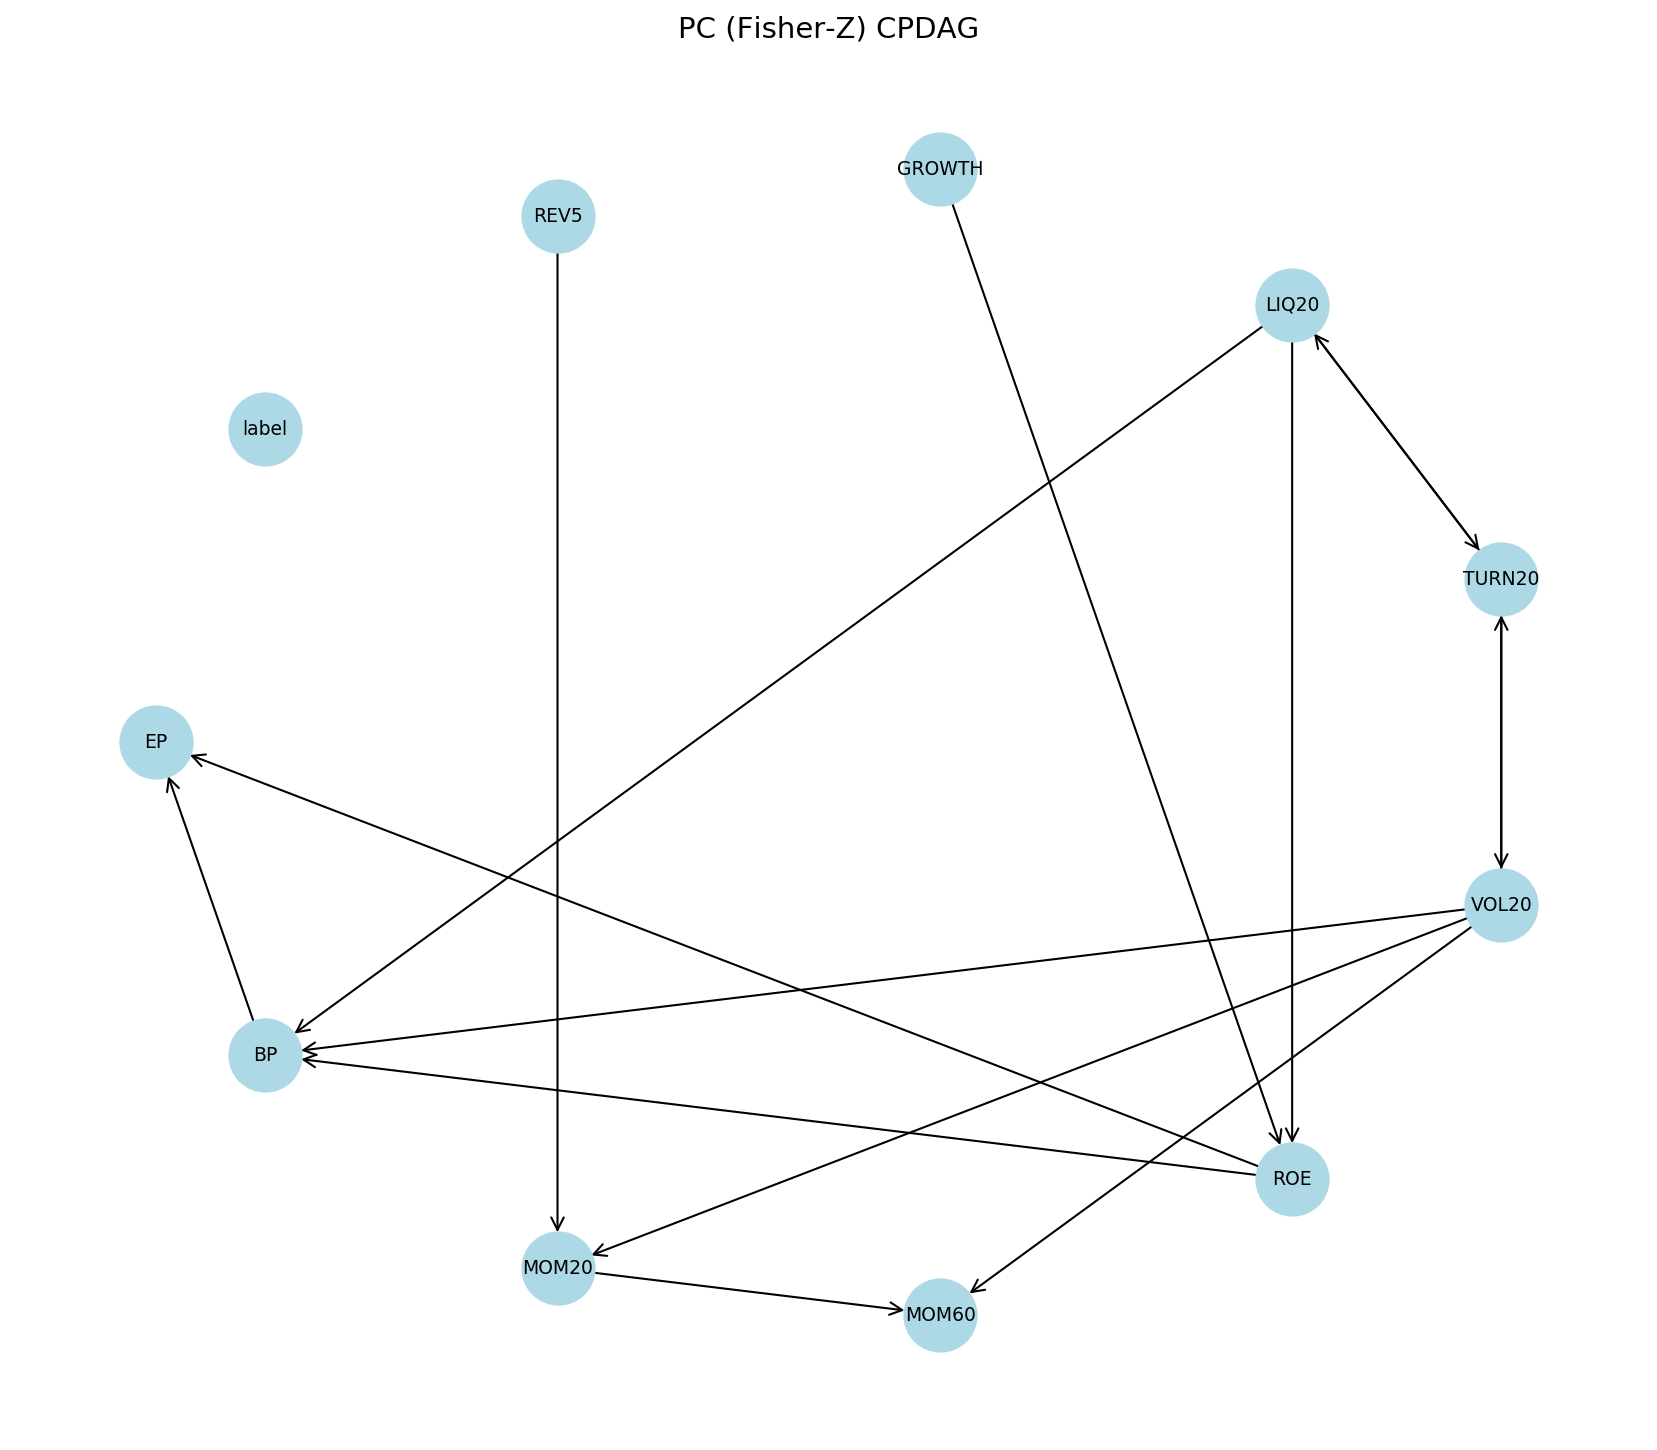
\includegraphics[width=0.95\textwidth]{figures/pc_dag.png}
\caption{PC 算法学习到的因果图（CPDAG）}
\end{figure}

\begin{figure}[htbp]
\centering
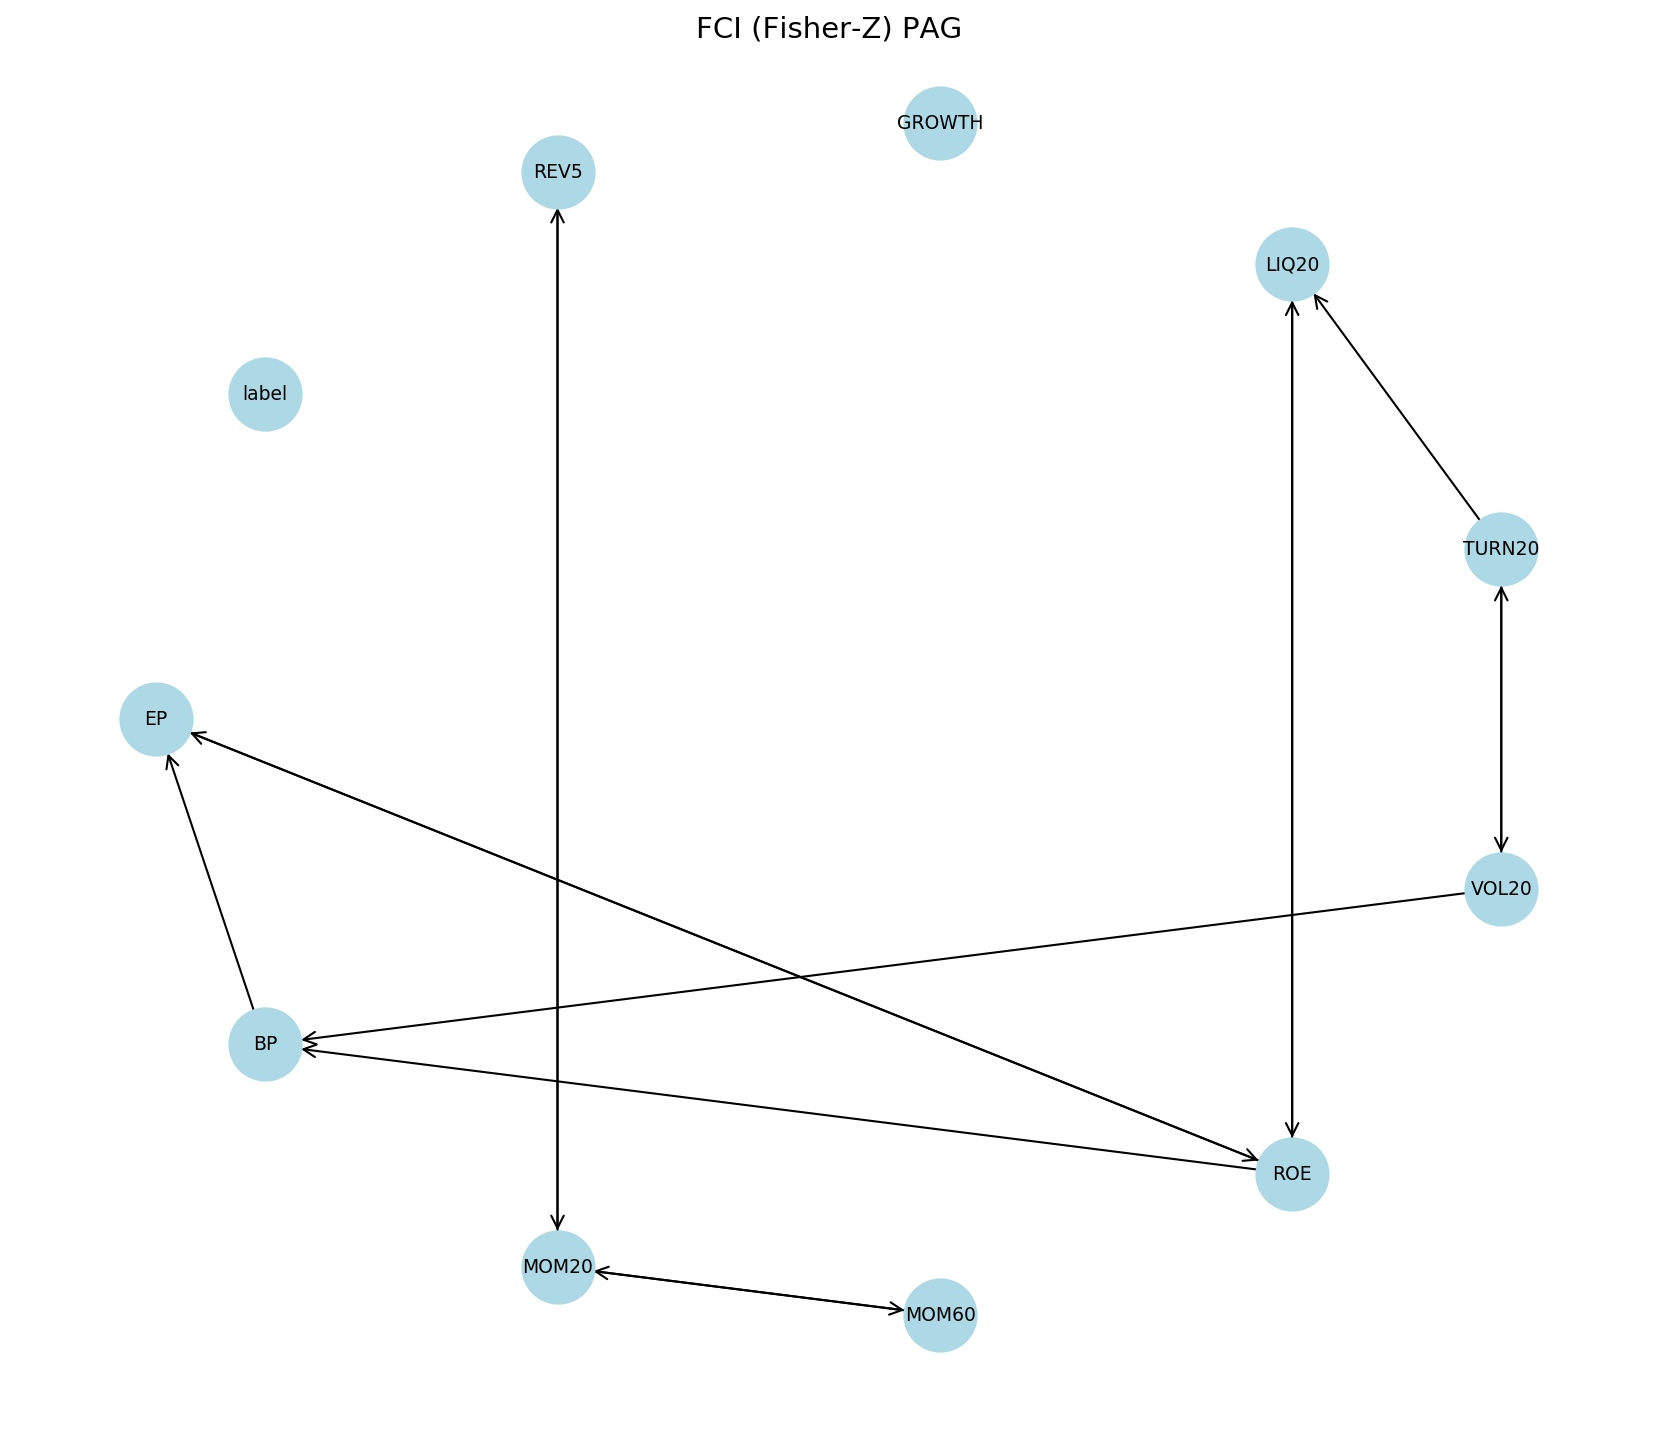
\includegraphics[width=0.95\textwidth]{figures/fci_pag.png}
\caption{FCI 算法学习到的部分祖先图（PAG）}
\end{figure}

\subsection{Bootstrap稳定性}
对真实数据进行 1000 次 Bootstrap 重采样，同时运行 PC 与 FCI 算法，报告每条边出现频率。仅保留稳定性 $> 70\%$ 的边。本次共识别 0 条稳定边。

\begin{figure}[htbp]
\centering
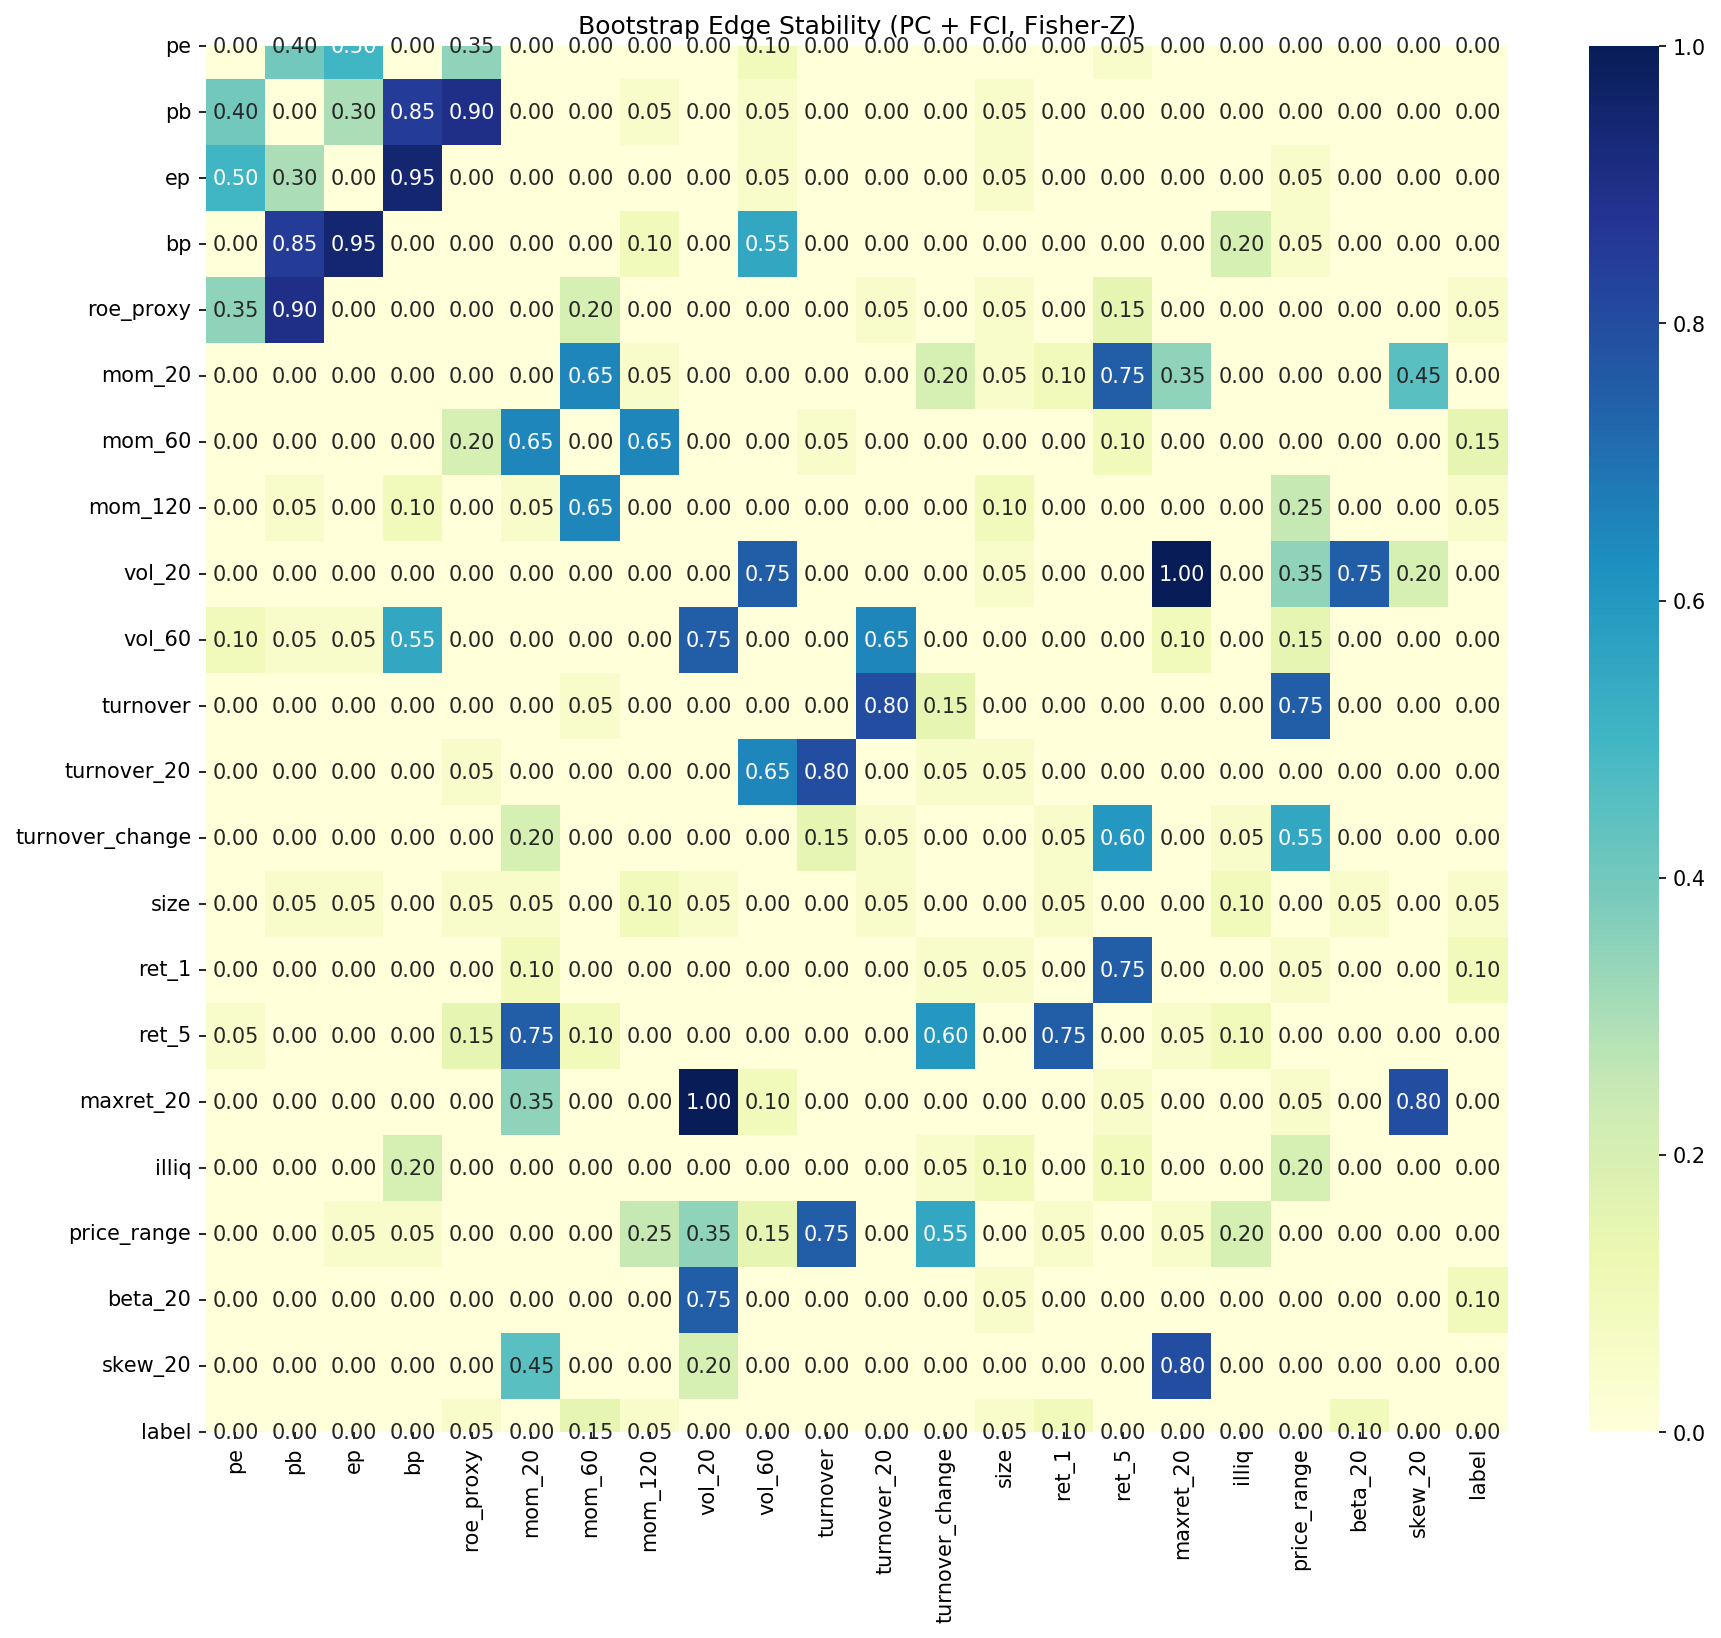
\includegraphics[width=0.95\textwidth]{figures/bootstrap_stability_heatmap.png}
\caption{Bootstrap 边稳定性热力图}
\end{figure}

\section{因果效应估计：四维方法矩阵}
对每个因子分别采用四种识别策略，比较因果效应值（ATE）与置信区间。若多方法一致，则因果效应更稳健。

\subsection{Double Machine Learning}
DML 使用 XGBoost 估计 $E[Y\mid X]$ 与 $E[D\mid X]$，通过 5-fold 交叉拟合残差化后回归。结果见表 \ref{tab:dml}。

\begin{table}[htbp]
\centering
\caption{DML 因果效应估计}
\label{tab:dml}
\begin{tabular}{ccccccc}
\toprule
factor & ate & se & tvalue & pvalue & ci\_lower & ci\_upper \\ 
\midrule
EP & -0.0061 & 0.0071 & -0.8644 & 0.3876 & -0.0200 & 0.0078 \\ 
BP & -0.0010 & 0.0064 & -0.1558 & 0.8762 & -0.0137 & 0.0116 \\ 
MOM20 & -0.0045 & 0.0037 & -1.2132 & 0.2253 & -0.0117 & 0.0028 \\ 
MOM60 & -0.0050 & 0.0037 & -1.3710 & 0.1706 & -0.0122 & 0.0022 \\ 
ROE & -0.0069 & 0.0060 & -1.1530 & 0.2491 & -0.0186 & 0.0048 \\ 
ROA & -0.0069 & 0.0060 & -1.1530 & 0.2491 & -0.0186 & 0.0048 \\ 
VOL20 & 0.0063 & 0.0045 & 1.3941 & 0.1635 & -0.0026 & 0.0152 \\ 
TURN20 & 0.0195 & 0.0045 & 4.3022 & 0.0000 & 0.0106 & 0.0284 \\ 
LIQ20 & -0.0049 & 0.0044 & -1.1112 & 0.2667 & -0.0136 & 0.0038 \\ 
GROWTH & 0.0019 & 0.0034 & 0.5500 & 0.5824 & -0.0049 & 0.0087 \\ 
REV5 & 0.0017 & 0.0033 & 0.5109 & 0.6095 & -0.0048 & 0.0082 \\ 
\bottomrule
\end{tabular}
\end{table}

\subsection{工具变量法（IV）}
构造行业均值 EP 与滞后一期因子作为工具变量。第一阶段 F 统计量需大于 10 以排除弱工具变量问题；Sargan 检验用于过度识别约束。结果见表 \ref{tab:iv}。

\begin{table}[htbp]
\centering
\caption{IV 因果效应估计}
\label{tab:iv}
\begin{tabular}{cccccc}
\toprule
factor & ate & se & pvalue & first\_stage\_f & sargan\_pvalue \\ 
\midrule
EP & -0.0099 & 0.0064 & 0.1200 & 2678.6488 & 0.6038 \\ 
BP & 0.0069 & 0.0066 & 0.2932 & 12733.2696 & 0.9998 \\ 
MOM20 & -0.0239 & 0.0091 & 0.0085 & 115.4584 & 0.2545 \\ 
MOM60 & -0.0246 & 0.0058 & 0.0000 & 428.8916 & 0.6101 \\ 
ROE & -0.0064 & 0.0057 & 0.2674 & 2211.4614 & 0.0780 \\ 
ROA & -0.0064 & 0.0057 & 0.2674 & 2211.4614 & 0.0780 \\ 
VOL20 & -0.0139 & 0.0138 & 0.3120 & 60.5847 & 0.4218 \\ 
TURN20 & 0.0194 & 0.0066 & 0.0035 & 808.7720 & 0.0241 \\ 
LIQ20 & -0.0093 & 0.0053 & 0.0784 & 2980.1467 & 0.8166 \\ 
GROWTH & 0.0064 & 0.0047 & 0.1768 & 1029.4862 & 0.1550 \\ 
REV5 & 0.0198 & 0.0109 & 0.0690 & 61.1991 & 0.0017 \\ 
\bottomrule
\end{tabular}
\end{table}

\subsection{前门调整}
以 5 日未来收益作为中介变量，通过两步估计识别 EP 到 20 日收益的因果效应。结果见表 \ref{tab:fd}。

\begin{table}[htbp]
\centering
\caption{前门调整因果效应估计}
\label{tab:fd}
\begin{tabular}{cccccc}
\toprule
factor & ate & se & pvalue & beta1 & beta2 \\ 
\midrule
EP & -0.0015 & 0.0022 & 0.4934 & -0.0017 & 0.9061 \\ 
BP & -0.0015 & 0.0023 & 0.5353 & -0.0016 & 0.9061 \\ 
MOM20 & 0.0011 & 0.0015 & 0.4483 & 0.0013 & 0.9061 \\ 
MOM60 & -0.0030 & 0.0015 & 0.0466 & -0.0033 & 0.9061 \\ 
ROE & 0.0018 & 0.0020 & 0.3465 & 0.0020 & 0.9061 \\ 
ROA & 0.0018 & 0.0020 & 0.3465 & 0.0020 & 0.9061 \\ 
VOL20 & -0.0036 & 0.0017 & 0.0350 & -0.0040 & 0.9061 \\ 
TURN20 & -0.0003 & 0.0018 & 0.8707 & -0.0003 & 0.9061 \\ 
LIQ20 & -0.0005 & 0.0017 & 0.7699 & -0.0006 & 0.9061 \\ 
GROWTH & 0.0007 & 0.0014 & 0.5967 & 0.0008 & 0.9061 \\ 
REV5 & -0.0013 & 0.0014 & 0.3433 & -0.0014 & 0.9061 \\ 
\bottomrule
\end{tabular}
\end{table}

\subsection{Causal Forest}
估计异质性处理效应（ITE），给出因子因果效应的截面分布。结果见表 \ref{tab:cf}。

\begin{table}[htbp]
\centering
\caption{Causal Forest 因果效应估计}
\label{tab:cf}
\begin{tabular}{ccccc}
\toprule
factor & ate & se & pvalue & ite\_std \\ 
\midrule
EP & -0.0061 & 0.0070 & 0.3876 & 0.4397 \\ 
BP & -0.0010 & 0.0064 & 0.8775 & 0.6353 \\ 
MOM20 & -0.0045 & 0.0037 & 0.2203 & 0.8265 \\ 
MOM60 & -0.0050 & 0.0037 & 0.1738 & 0.5844 \\ 
ROE & -0.0070 & 0.0059 & 0.2361 & 0.5135 \\ 
ROA & -0.0070 & 0.0059 & 0.2361 & 0.4965 \\ 
VOL20 & 0.0065 & 0.0045 & 0.1532 & 0.4418 \\ 
TURN20 & 0.0195 & 0.0045 & 0.0000 & 0.4776 \\ 
LIQ20 & -0.0049 & 0.0044 & 0.2683 & 0.6394 \\ 
GROWTH & 0.0019 & 0.0034 & 0.5714 & 0.5537 \\ 
REV5 & 0.0016 & 0.0033 & 0.6300 & 0.7601 \\ 
\bottomrule
\end{tabular}
\end{table}

\begin{figure}[htbp]
\centering
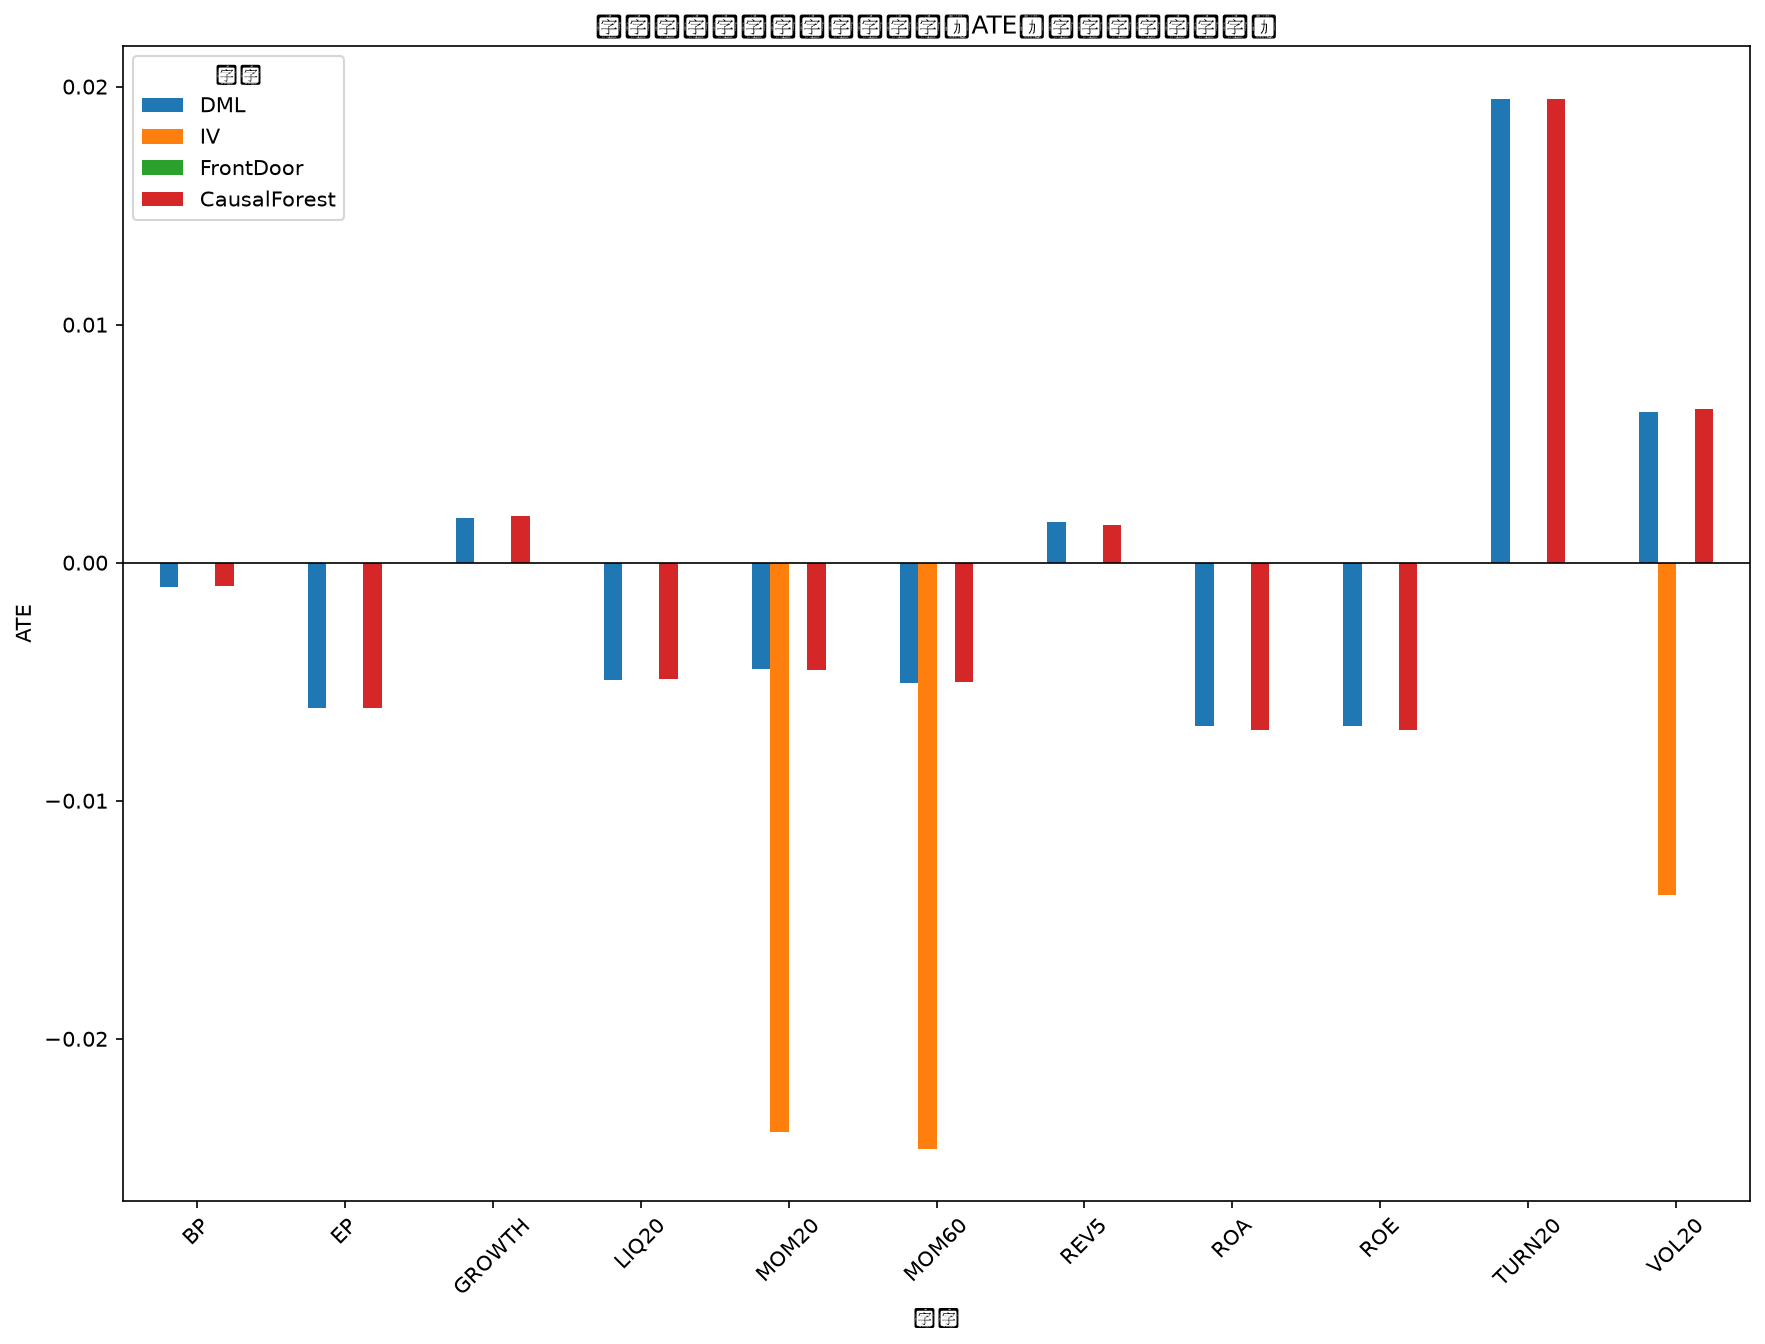
\includegraphics[width=0.95\textwidth]{figures/causal_effect_comparison.png}
\caption{四种方法 ATE 对比}
\end{figure}

\section{因果因子 vs 相关因子}
\subsection{2$\times$2 分类矩阵}
按因果显著性（四种方法中至少两种显著且符号一致）与训练集 IC 显著性（$|t|>2$）交叉分类：
\begin{itemize}
    \item \textbf{因果显著 \& IC显著}：真因子
    \item \textbf{因果显著 \& IC不显著}：被掩盖的因子
    \item \textbf{因果不显著 \& IC显著}：伪因子（由混杂驱动的虚假相关）
    \item \textbf{均不显著}：无效因子
\end{itemize}

\begin{table}[htbp]
\centering
\caption{因子 2$\times$2 分类矩阵}
\label{tab:matrix}
\begin{tabular}{lcc}
\toprule
 & IC显著 & IC不显著 \\ 
\midrule
因果显著 & 0 & 3 \\ 
因果不显著 & 1 & 7 \\ 
\bottomrule
\end{tabular}
\end{table}

因果显著因子：\texttt{['MOM20', 'MOM60', 'TURN20']}。\\
IC 显著因子：\texttt{['ROE']}。\\
伪因子（IC 显著但因果不显著）：\texttt{['ROE']}。\\
被掩盖的因子（因果显著但 IC 不显著）：\texttt{['MOM20', 'MOM60', 'TURN20']}。

\subsection{IC 衰减曲线}
在 2023--2024 年测试集上计算滚动 IC，对比因果显著组、IC 显著组与其他组的衰减。

\begin{figure}[htbp]
\centering
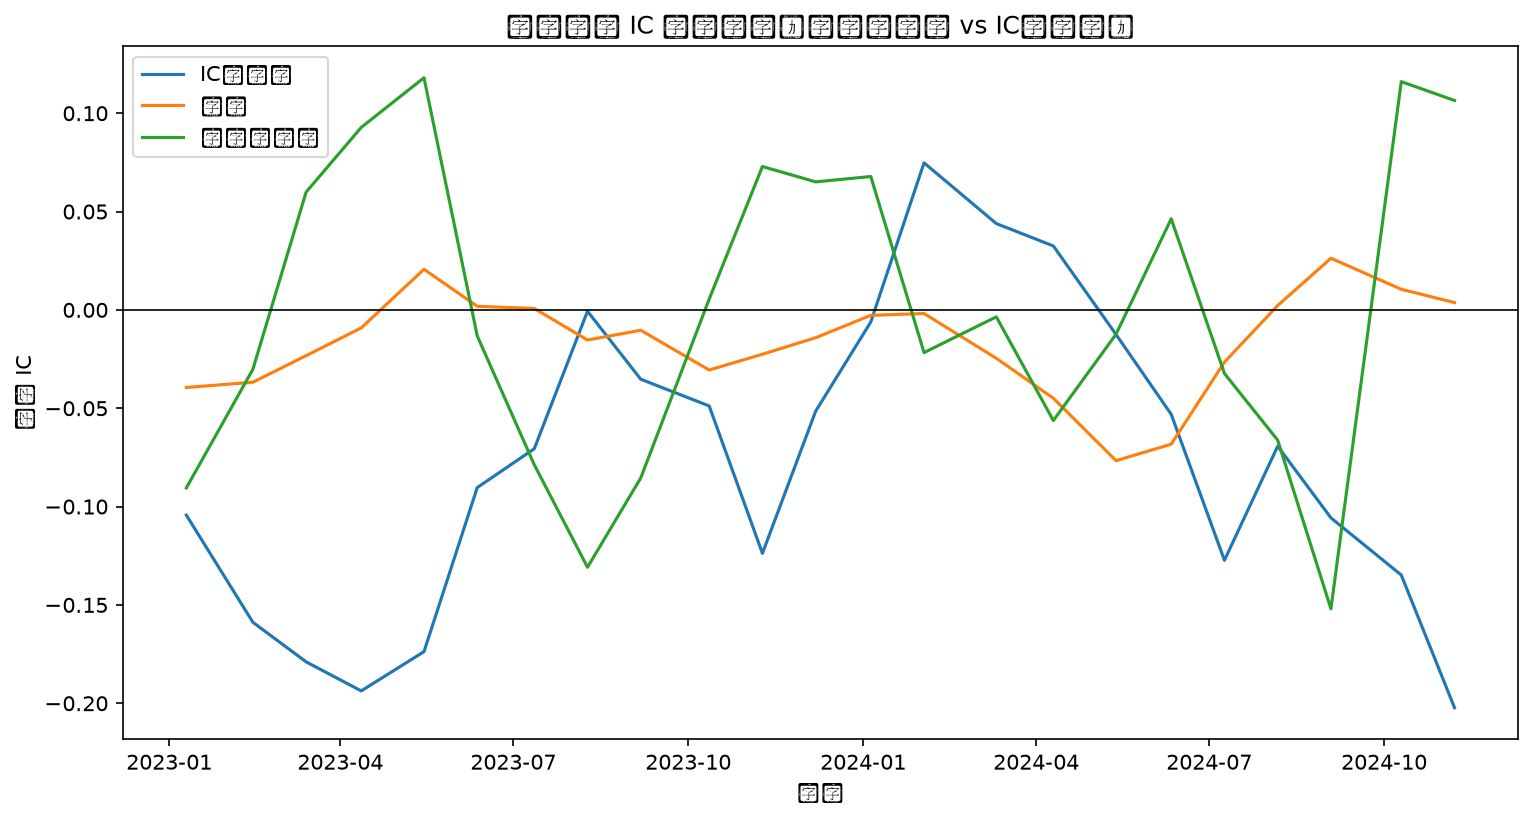
\includegraphics[width=0.95\textwidth]{figures/ic_decay_curves.png}
\caption{因子滚动 IC 衰减曲线}
\end{figure}

\begin{table}[htbp]
\centering
\caption{因子 IC 衰减率}
\label{tab:decay}
\begin{tabular}{ccccccc}
\toprule
factor & group & first\_half\_ic & second\_half\_ic & raw\_decay\_rate & decay\_rate & stability\_score \\ 
\midrule
EP & 其他 & 0.0146 & 0.0247 & -0.6971 & 0.0000 & 1.0000 \\ 
BP & 其他 & 0.0613 & 0.0332 & 0.4583 & 0.4583 & 0.5417 \\ 
MOM20 & 因果显著组 & 0.0012 & 0.0240 & -18.8437 & 0.0000 & 1.0000 \\ 
MOM60 & 因果显著组 & 0.0073 & 0.0326 & -3.4872 & 0.0000 & 1.0000 \\ 
ROE & IC显著组 & -0.1072 & -0.0510 & 0.5246 & 0.5246 & 0.4754 \\ 
ROA & 其他 & -0.1072 & -0.0510 & 0.5246 & 0.5246 & 0.4754 \\ 
VOL20 & 其他 & -0.0664 & -0.0550 & 0.1718 & 0.1718 & 0.8282 \\ 
TURN20 & 因果显著组 & -0.0302 & -0.0423 & -0.3981 & 0.0000 & 1.0000 \\ 
LIQ20 & 其他 & 0.0258 & -0.0208 & 0.1945 & 0.1945 & 0.8055 \\ 
GROWTH & 其他 & -0.0532 & -0.0214 & 0.5967 & 0.5967 & 0.4033 \\ 
REV5 & 其他 & 0.0206 & -0.0363 & -0.7661 & 0.0000 & 1.0000 \\ 
\bottomrule
\end{tabular}
\end{table}

\subsection{因子拥挤度}
以因子横截面标准差衡量拥挤度，比较高低拥挤度下的 IC 差异。

\begin{figure}[htbp]
\centering
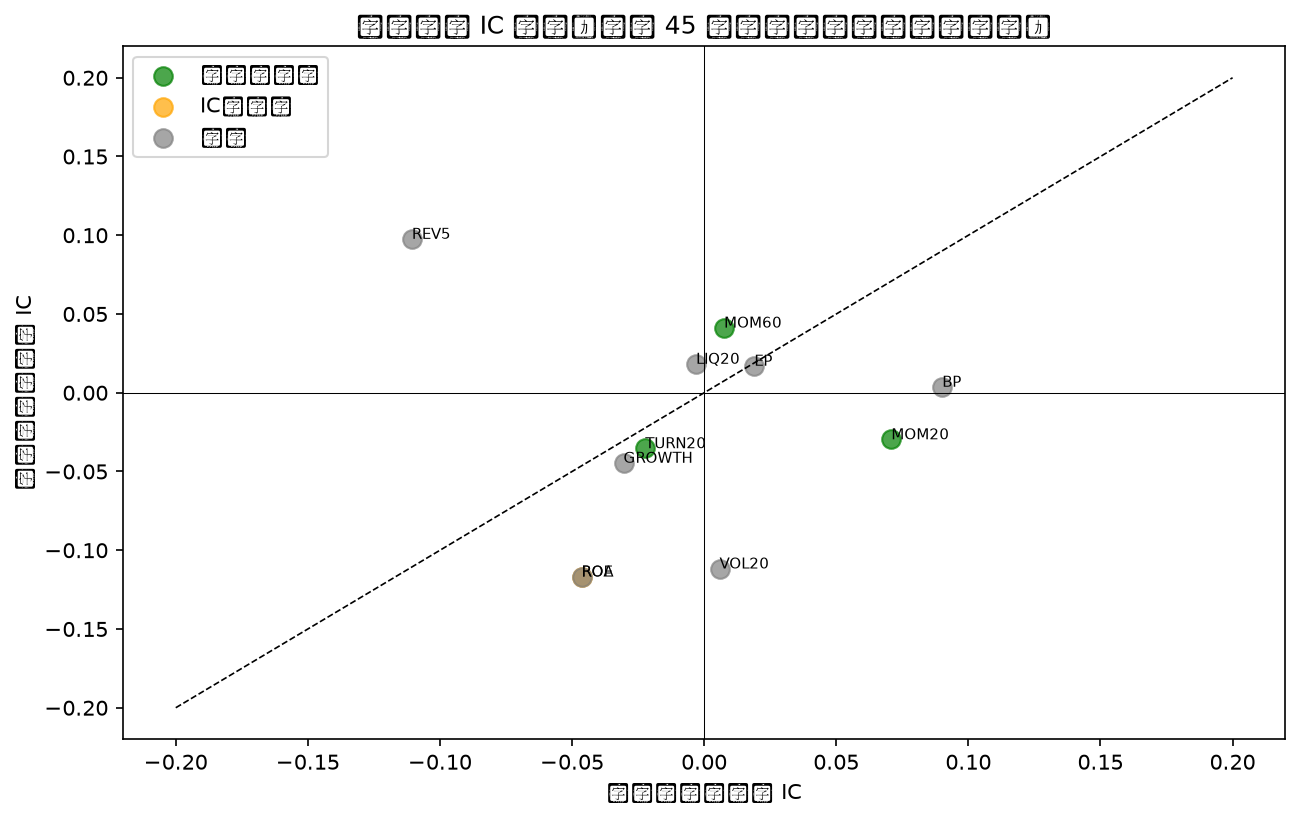
\includegraphics[width=0.95\textwidth]{figures/crowding_ic.png}
\caption{拥挤度与 IC 关系}
\end{figure}

\section{组合回测}
在 2023--2024 年样本外，比较三组多空组合：全因子等权、IC 显著因子、因果显著因子。每组选择因子得分最高/最低的 30 只股票，等权做多/做空，计入交易成本。

\begin{figure}[htbp]
\centering
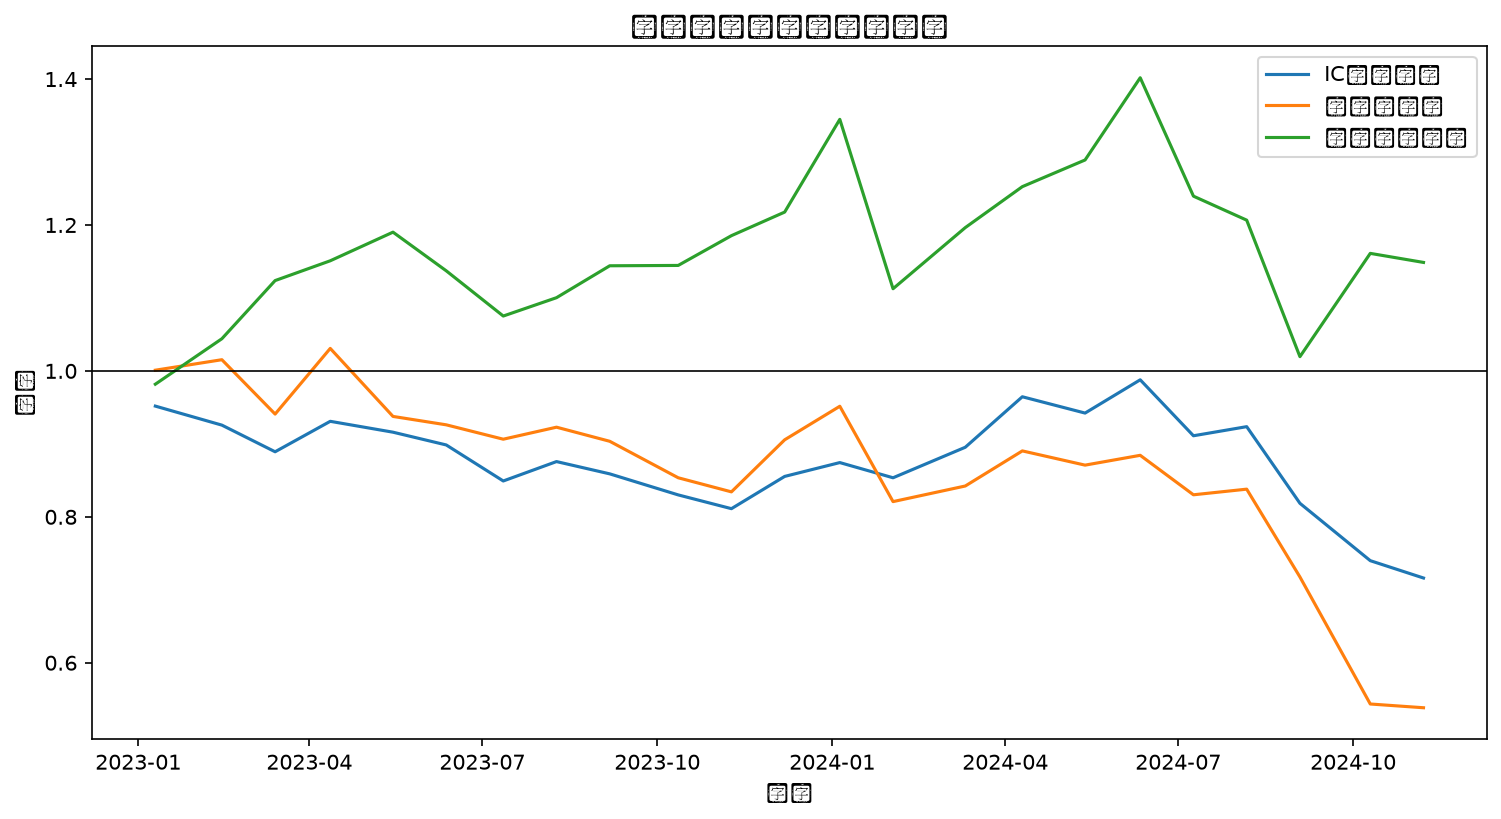
\includegraphics[width=0.95\textwidth]{figures/backtest_nav_curves.png}
\caption{三组组合样本外净值曲线}
\end{figure}

\begin{figure}[htbp]
\centering
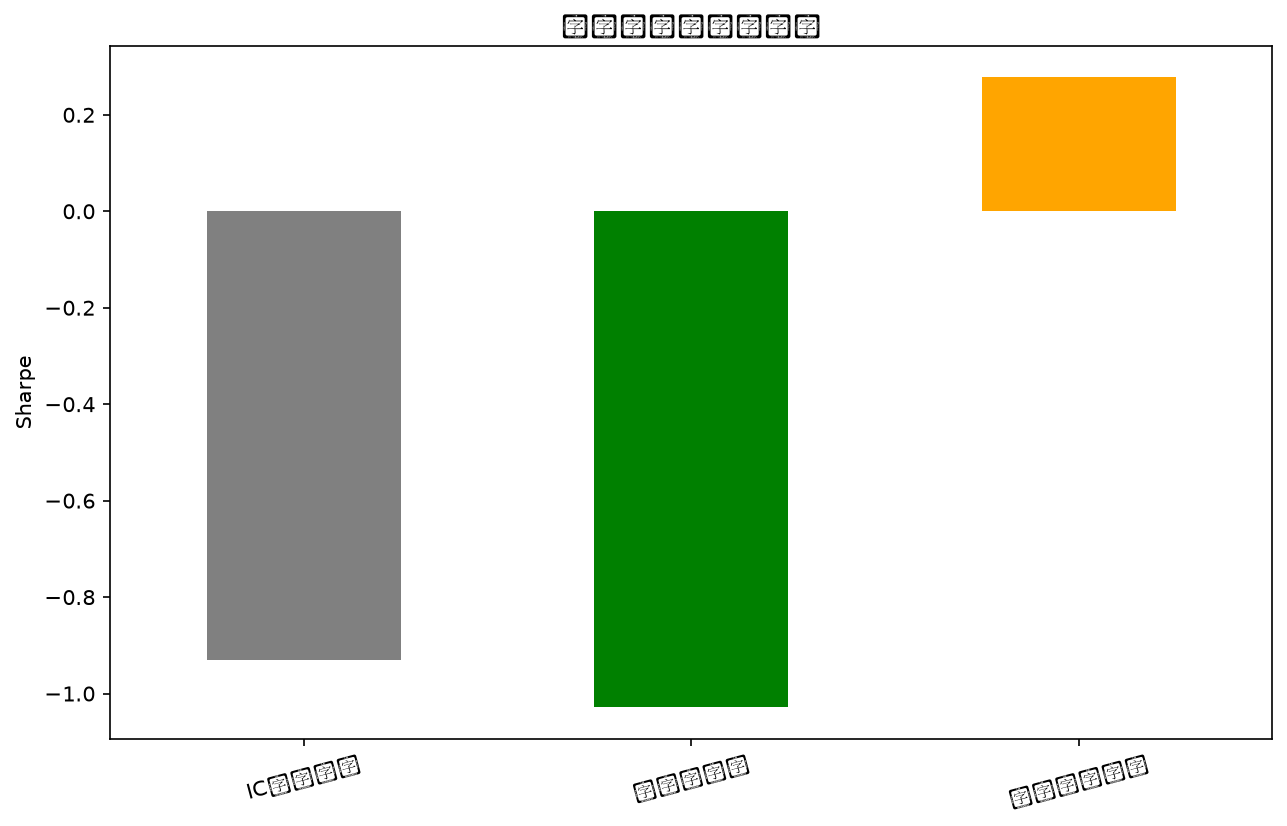
\includegraphics[width=0.95\textwidth]{figures/backtest_sharpe_comparison.png}
\caption{样本外夏普比率对比}
\end{figure}

\begin{table}[htbp]
\centering
\caption{组合回测绩效指标}
\label{tab:backtest}
\begin{tabular}{cccccccccc}
\toprule
组合 & annual\_return & annual\_vol & sharpe & max\_drawdown & win\_rate & total\_return & calmar & information\_ratio & sortino \\ 
\midrule
IC显著因子 & -0.1599 & 0.1719 & -0.9302 & -0.2750 & 0.3478 & -0.2839 & -0.5813 & -0.6407 & -1.5329 \\ 
全因子等权 & -0.2761 & 0.2684 & -1.0286 & -0.4778 & 0.4348 & -0.4617 & -0.5779 & -0.7594 & -1.1583 \\ 
因果显著因子 & 0.0750 & 0.2701 & 0.2777 & -0.2727 & 0.6522 & 0.1487 & 0.2750 & 0.0181 & 0.3383 \\ 
\bottomrule
\end{tabular}
\end{table}

\section{稳健性检验}
\subsection{Rosenbaum 敏感性边界}
检验因果结论对未观测混杂的稳健性。$\Gamma$ 从 1.0 增加到 2.0，若 $\Gamma=1.5$ 时仍显著则为中等稳健，$\Gamma=2.0$ 仍显著则为高度稳健。

\begin{figure}[htbp]
\centering
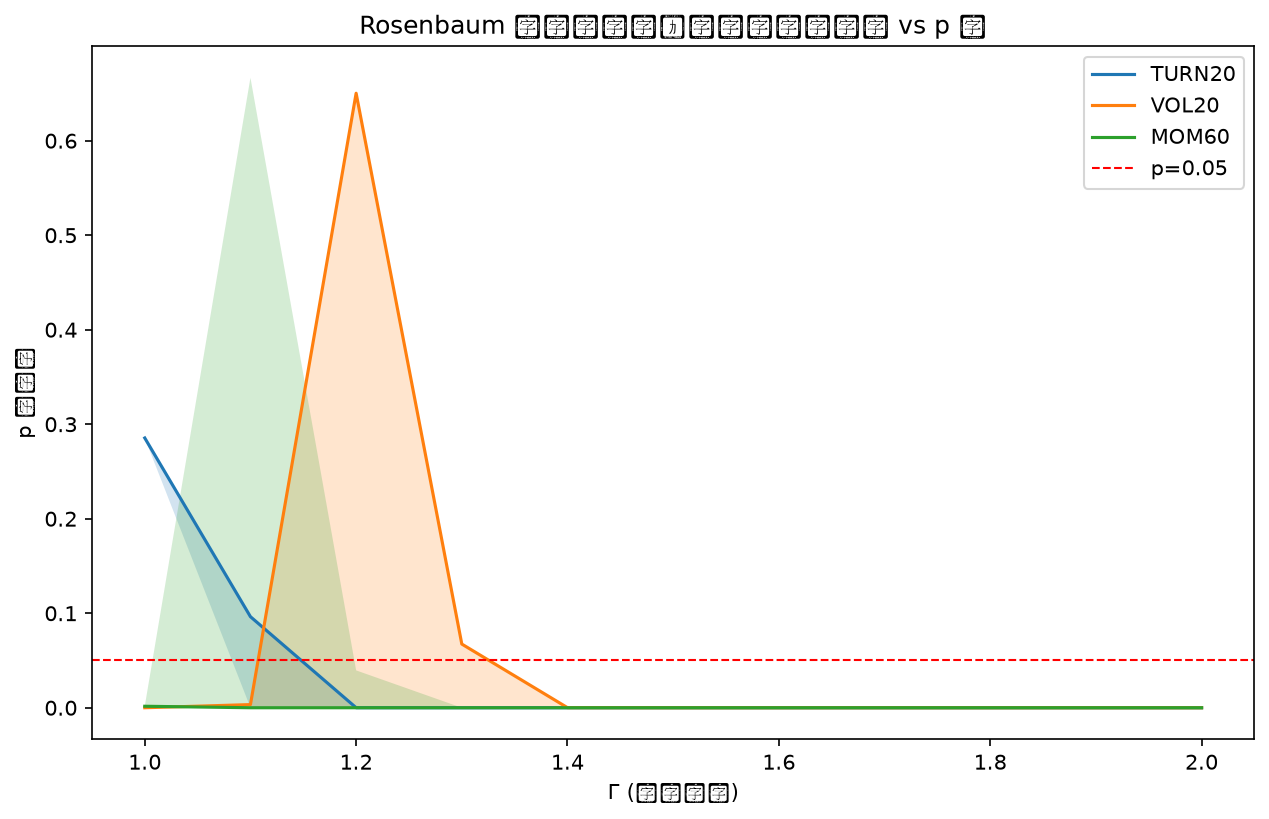
\includegraphics[width=0.95\textwidth]{figures/rosenbaum_bounds.png}
\caption{Rosenbaum 敏感性边界}
\end{figure}

\subsection{Placebo 检验}
对随机噪声因子与截面打乱后的真实因子运行完整因果推断流程，预期伪因子因果效应不显著。

\begin{table}[htbp]
\centering
\caption{Placebo 检验结果}
\label{tab:placebo}
\begin{tabular}{ccccccccc}
\toprule
placebo\_type & method & n\_seeds & n\_sig\_raw & fpr\_raw & n\_sig\_fdr & n\_sig\_valid & binom\_test\_pvalue & fpr\_inflated \\ 
\midrule
noise & CausalForest & 20.0000 & 1.0000 & 0.0500 & 0.0000 & 1.0000 & 0.6415 & 0.0000 \\ 
noise & DML & 20.0000 & 1.0000 & 0.0500 & 0.0000 & 1.0000 & 0.6415 & 0.0000 \\ 
noise & FrontDoor & 20.0000 & 3.0000 & 0.1500 & 0.0000 & 1.0000 & 0.0755 & 0.0000 \\ 
noise & IV & 20.0000 & 2.0000 & 0.1000 & 0.0000 & 1.0000 & 0.2642 & 0.0000 \\ 
shuffled & CausalForest & 20.0000 & 1.0000 & 0.0500 & 0.0000 & 1.0000 & 0.6415 & 0.0000 \\ 
shuffled & DML & 20.0000 & 1.0000 & 0.0500 & 0.0000 & 1.0000 & 0.6415 & 0.0000 \\ 
shuffled & FrontDoor & 20.0000 & 0.0000 & 0.0000 & 0.0000 & 0.0000 & 1.0000 & 0.0000 \\ 
shuffled & IV & 20.0000 & 1.0000 & 0.0500 & 0.0000 & 1.0000 & 0.6415 & 0.0000 \\ 
\bottomrule
\end{tabular}
\end{table}

\subsection{时间置换检验}
将因子向前平移一期，检验未来因子是否因果影响当前收益。预期结果不显著。

\begin{table}[htbp]
\centering
\caption{时间置换检验结果}
\label{tab:timeperm}
\begin{tabular}{cccc}
\toprule
factor & ate & pvalue & tvalue \\ 
\midrule
EP & -0.0362 & 0.0000 & -5.6947 \\ 
BP & -0.0353 & 0.0000 & -5.6463 \\ 
MOM20 & 0.0945 & 0.0000 & 55.9877 \\ 
MOM60 & 0.0723 & 0.0000 & 23.3189 \\ 
ROE & -0.0053 & 0.3408 & -0.9530 \\ 
ROA & -0.0053 & 0.3408 & -0.9530 \\ 
VOL20 & 0.0343 & 0.0000 & 9.3069 \\ 
TURN20 & 0.0374 & 0.0000 & 9.4091 \\ 
LIQ20 & 0.0040 & 0.3439 & 0.9469 \\ 
GROWTH & 0.0042 & 0.2097 & 1.2549 \\ 
REV5 & -0.0522 & 0.0000 & -19.1234 \\ 
\bottomrule
\end{tabular}
\end{table}

\subsection{分市场状态}
按市场趋势将样本划分为熊市、震荡市与牛市，分别估计 DML 因果效应。

\begin{figure}[htbp]
\centering
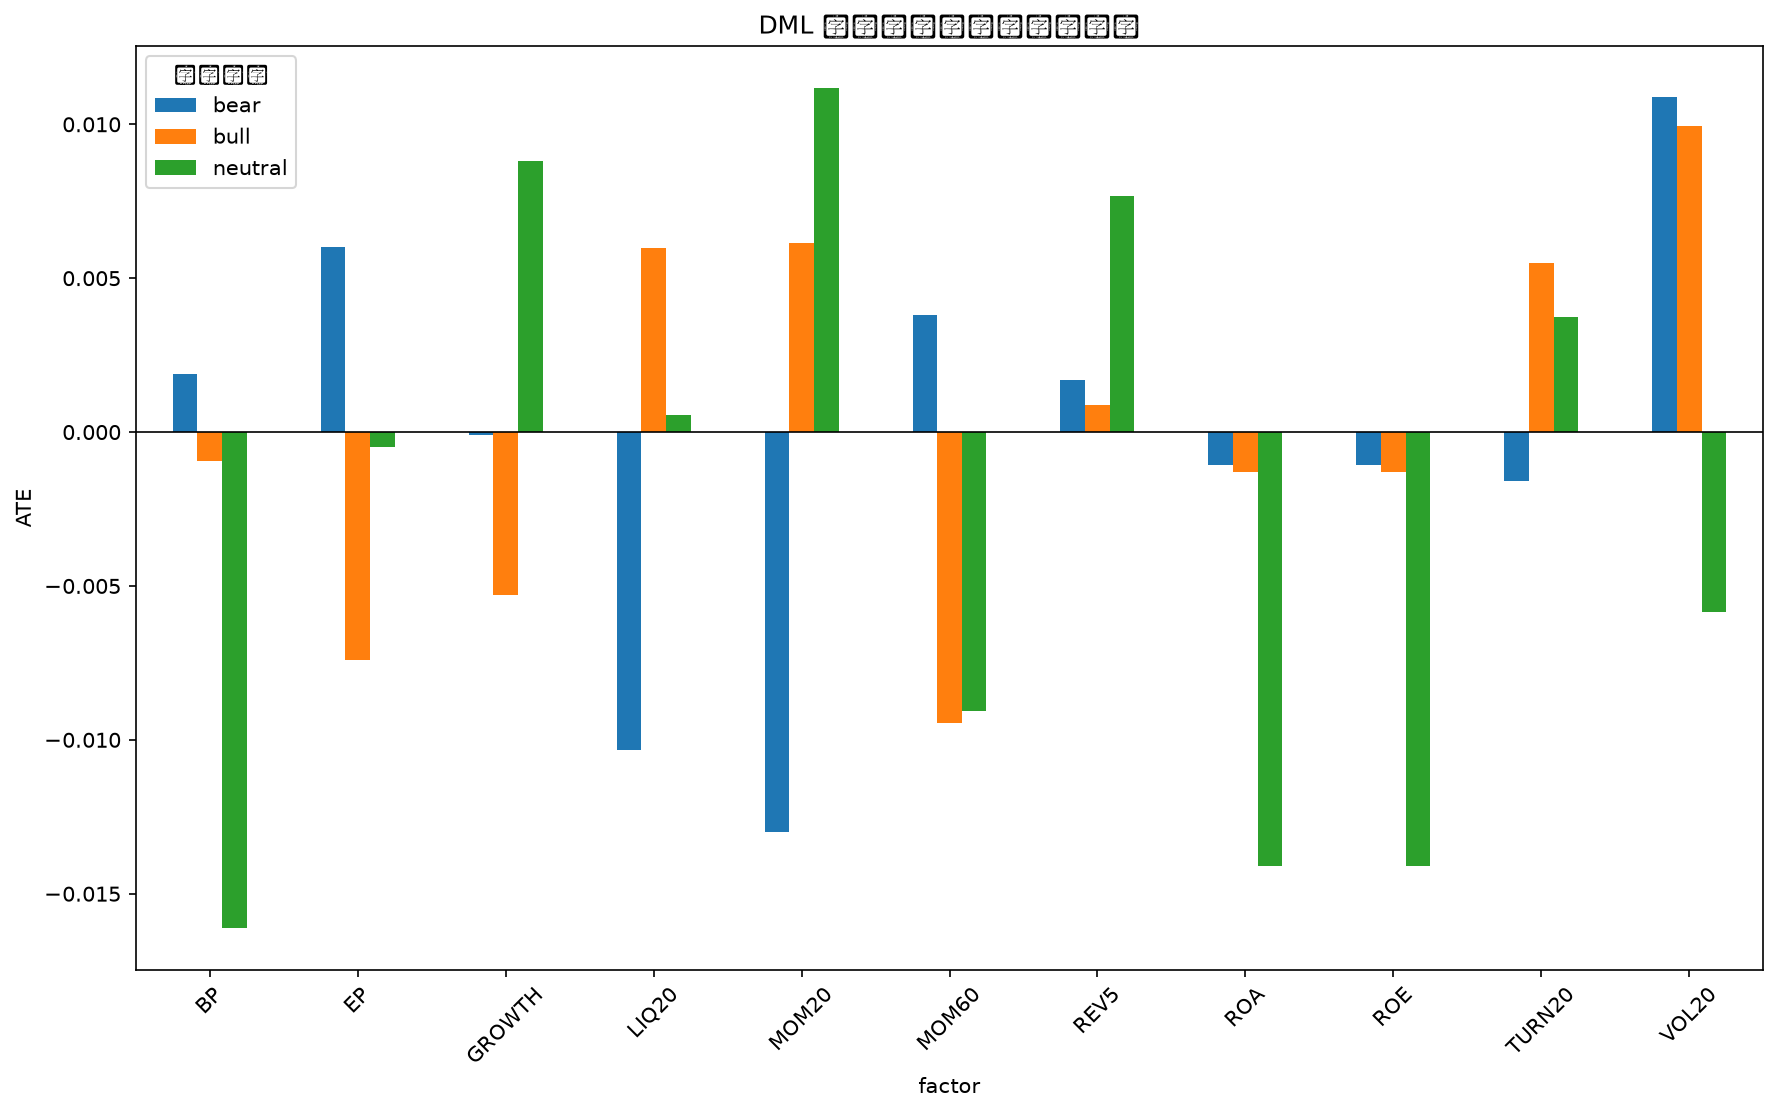
\includegraphics[width=0.95\textwidth]{figures/market_regime_comparison.png}
\caption{DML 因果效应分市场状态对比}
\end{figure}

\section{数学严谨性：do-演算与识别假设}
\subsection{后门准则与 do-演算}
若控制变量集 $Z$ 阻断了从处理 $D$ 到结果 $Y$ 的所有后门路径，则
\begin{equation}
P(Y \mid do(D=d)) = \sum_z P(Y \mid D=d, Z=z) P(Z=z)
\end{equation}

本研究对每个因子纳入行业、市值、动量、波动率等控制变量以阻断后门路径。倾向得分重叠度平均为 0.8852，共同支撑条件 良好。

\subsection{识别假设}
\begin{itemize}
    \item \textbf{可忽略性}：给定控制变量 $Z$，处理分配（因子暴露）与潜在结果（未来收益）近似独立。未观测的市场情绪、宏观冲击仍可能构成残余混杂。
    \item \textbf{共同支撑域}：处理组与对照组在控制变量上存在重叠，通过倾向得分分布验证。
    \item \textbf{SUTVA}：横截面因子研究中个股处理效应近似独立，但因子组合内股票间可能存在溢出效应。SUTVA 风险较高的因子：\texttt{['EP', 'BP', 'MOM20', 'MOM60', 'ROE', 'VOL20', 'TURN20', 'LIQ20', 'REV5']}。
\end{itemize}

\section{结论与局限}
部分传统 IC 显著因子（如 ROE）在因果推断中并不显著，存在伪因子风险。 因果显著因子包括：MOM20, MOM60, TURN20。 因果显著因子组合样本外夏普（0.2777）高于 IC 显著因子组合（-0.9302），支持因果因子更稳健的判断。

本研究的主要局限包括：工具变量的排除性约束无法直接验证，前门调整的中介变量为代理变量，未观测混杂无法完全排除，以及因果发现算法对分布假设和样本量敏感。未来工作可探索更大样本、更精细的中介变量与动态因果图方法。

\bibliographystyle{plain}
\bibliography{references}

\end{document}
